\chapter{Detecção de fraude}

A fraude pode ter origem tanto interna quanto externa a uma organização. Por exemplo, uma empresa está sujeita a fraude por seus administradores (denominada de alto-nível) ou empregados que não sejam gestores (baixo-nível) \cite{Phua2010}. Em um documento de 2012, a Associação de Investigadores Certificados de Fraude (Association of Certified Fraud Examiners, ACFE) definiu a fraude interna como a exploração ilegal dos recursos e bens de uma empresa, por um empregado, para enriquecimento próprio \cite{ACFE2012}.

Já na fraude externa, os seus autores dividem-se em três perfis: casual, criminal e crime organizado \cite{Phua2010}. Criminosos casuais apresentam comportamento aleatório, transgredindo as leis quando têm oportunidade, tentação ou em períodos de dificuldades financeiras. Por outro lado, indivíduos ou grupos organizados são mais perigosos porque tentam esconder ou dissimular sua verdadeira identidade, além de evoluir seu \emph{modus operandi} com o tempo, tentando burlar os sistemas de detecção e evitar a sua identificação. Assim, é importante levar-se em consideração essa constante interação entre os sistemas de detecção e os fraudadores profissionais. Essas categorias de fraudadores geralmente atuam em um setor específico: as fraudes internas e de seguro são mais frequentemente exploradas por criminosos comuns, enquanto fraudes de cartão de crédito e telecomunicações são vítimas de fraudadores profissionais.

O monitoramento de sistemas com o objetivo de encontrar comportamentos fraudulentos já existia muito antes da utilização dos sistemas computacionais tornarem-se ferramentas comuns. Antes havia um processo denominado auditoria: gerar, armazenar e revisar um registro cronológico de eventos de um sistema \cite{Bace2000}. Os principais objetivos dos sistemas de auditoria são identificar os usuários do sistema, impedir o uso impróprio, e auxiliar na reconstrução de eventos e na estimativa, quantificação e qualificação de danos.

O primeiro trabalho a considerar necessária a auditoria automática de sistemas foi \citet{Anderson1972}. Nesse trabalho, Anderson classifica os riscos e ameaças a sistemas, diferenciando fontes internas e externas, como na figura \ref{fraud:and}. Ele também cita diversos objetivos para um sistema de auditoria:

\begin{enumerate}[a)]
    \item Prover informações suficientes para que o problema possa ser localizado, mas que não exponham detalhes que possibilitem um ataque.
    \item Obter dados de diversas fontes para otimizar o conteúdo do banco de dados.
    \item Discernir uma atividade ``normal'' do sistema, para que se possa detectar abusos interno.
    \item Levar em consideração as estratégias dos invasores no projeto do sistema.
\end{enumerate}

A detecção de fraude é apenas uma das etapas de um sistema chamado de \emph{controle de fraude}. Nesse contexto, a detecção automática ajuda a reduzir o trabalho manual de verificação das instâncias \cite{Phua2010}. O objetivo principal desses sistemas é identificar padrões de transações suspeitas em meio às transações comuns de uma organização. O fraudador pode, por exemplo, contratar um seguro usando informações de outra pessoa ou informações falsas. O sistema procura detectar e impedir a fraude o mais cedo possível.

\renewcommand{\arraystretch}{1.5}
\begin{table}[h!]
    \vspace{0.5cm}
    \centering
    \caption{Matriz de ameaças}
    \label{fraud:and}
    \vspace{0.5cm}
    \begin{tabular}{c p{4cm}|>{\centering\arraybackslash}p{4cm}|>{\centering\arraybackslash}p{4cm}|}
        \cline{3-4}
        & & Uso não autorizado dos dados/programa & Uso autorizado dos dados/programa \\
        \hhline{~---}
        \multicolumn{0}{c|}{} & Uso não autorizado do computador & Invasão externa & \cellcolor{gray!90} \\
        \cline{2-4}
        \multicolumn{0}{c|}{} & Uso autorizado do computador & Invasão interna & Abuso de poder \\
        \cline{2-4}
    \end{tabular}
    \vspace{0.5cm}
    \\ Fonte: \cite{Anderson1972}.
    \vspace{0.5cm}
\end{table}

Geralmente não é possível ter absoluta certeza sobre a legitimidade das transações de um negócio a partir dos dados disponíveis. Não seria possível verificar todas as entidades com as quais uma empresa mantém relações, que em algumas empresas podem ser milhares. Assim, não existe uma técnica infalível para a detecção de fraudes. Isso não significa que elas não possam ser detectadas. A melhor alternativa, na prática, é uma busca por possíveis evidências de fraude nos dados disponíveis. Métodos matemáticos e estatísticos são utilizados para comparar um banco de dados de transações existentes com as novas, com o objetivo de encontrar evidências de possíveis fraudes. Mesmo assim, geralmente há um processo de análise e revisão caso a caso por um especialista.

Ainda, segundo a pesquisa apresentada no mesmo trabalho, o motor analítico desse tipo de sistema pode ser composto de um ou mais métodos, tais como: Sistemas Imunológicos Artificiais, inteligência artificial, auditoria, bancos de dados, computação distribuída e paralela, econometria, sistemas especialistas, lógica nebulosa, algoritmos genéticos, aprendizagem de máquina, redes neurais, reconhecimento de padrões, estatística, visualização, entre outros.

Dois conceitos relacionados à detecção em geral são falsos positivos e falsos negativos. Falsos positivos são instâncias erroneamente classificadas, por exemplo, uma transação comum que é classificada como fraudulenta. Falsos negativos são o oposto: uma transação fraudulenta que é classificada como comum. O número de falsos positivos aumenta o trabalho desnecessário na fase de revisão, enquanto os falsos negativos reduzem a eficácia da detecção.

A redução dos falsos positivos é um dos objetivos principais de um sistema de detecção. Os falsos negativos, no entanto, são quase impossíveis de serem eliminados completamente, em qualquer sistema de detecção \cite{Michie1994}. Mesmo um sistema capaz de reconhecer sinais de fraudes existentes não é suficiente para um ambiente real. Fraudadores tentam constantemente superar os sistemas de detecção, evoluindo o seu \emph{modus operandi} com o tempo, novos métodos são criados, novos fraudadores entram em atividade. Um sistema que almeje deter o maior número possível deve ser constantemente atualizado para se adaptar às mudanças de um ambiente tão dinâmico.

Dependendo do domínio da organização, para que um sistema possa prever fraudes com antecedência suficiente para que elas sejam evitadas, ele deve monitorar constantemente as novas transações em andamento. Esse fator reduz a utilização de sistemas que necessitam de um longo tempo de treinamento ou de análise. O ideal seria que ele estivesse em constante execução, analisando as transações conforme elas ocorrem. Para aplicações grandes ou descentralizadas, pode ser muito difícil conseguir isso sem afetar a performance geral das transações.

Para cada domínio, tipos diferentes de fraude podem existir, e mais de um tipo pode ocorrer simultaneamente, sem uma ordem definida.

\section{Dados}
\label{sec:fraud_data}

Existem alguns conceitos sobre as bases de dados que são característicos da área de mineração de dados e aprendizagem de máquina. O número de instâncias na base é chamado de número de \emph{amostras} e o número de atributos de cada instância é chamado de número de \emph{características} (em inglês, \emph{samples} e \emph{features}).

Os atributos das instâncias em um banco de dados usado para detecção de fraude geralmente limitam-se a valores binários, numéricos, categóricos ou uma mistura desses três. Os atributos específicos usados geralmente são semelhantes. Aplicações de seguro utilizam o histórico do cliente: tempo de contrato, histórico e total de pagamentos, lucro anual valor médio depositado em conta bancária. Para fraudes de crédito, utilizam-se informações sobre as transações: valor, data, localização geográfica, conta de destino, tempo de conta, etc. Fraudes em seguros de automóveis utilizam valores binários para atributos como acidente e tratamento hospitalar, além de dados do motorista, custo, tipo de ferimento, etc.

O número de instâncias positivas nas bases de dados de fraude é geralmente muito reduzido: as fraudes representam um percentual muito pequeno em relação ao número de transações legítimas de uma organização, geralmente menor do que 20\%. Métodos de detecção de fraude nunca são perfeitos: deve existir um mecanismo para lidar com as fraudes que não são identificadas a tempo de serem impedidas.

A obtenção de bancos de dados reais para teste é difícil, já que empresas e organizações, por razões legais e competitivas não disponibilizam informações desse tipo. Assim, é difícil encontrar bases de dados públicos para que os testes sejam realizados. Outra desvantagem comumente encontrada nesses bancos de dados é o fato dos dados estarem alterados, para a preservação da confidencialidade dos clientes das empresas fornecedoras. Apesar dos dados ainda poderem ser utilizados normalmente em ambientes de teste, não é possível, como seria caso se tivesse acesso aos dados originais, derivar regras de classificação dos resultados dos testes. Por exemplo, observando os resultados, seria possível perceber que um valor alto em um atributo leva a instância ser classificada como fraudulenta na maioria dos casos. Em uma base de dados esse atributo teria uma descrição informativa, mas isso é perdido em uma base alterada, onde ele seria descrito por um identificador sem significado, como ``atributo 5''.

Uma alternativa é a criação de um banco de dados artificial, inspirado em dados reais. A eficácia dessa técnica é limitada pela capacidade do criador do banco em prever o maior número de casos possíveis, o que geralmente é muito inferior à variedade das situações reais. Mesmo assim, essa técnica é comumente empregada na fase de concepção e teste, devido à dificuldade de obtenção de dados.

\section{Implementação}

A maioria dos sistemas de detecção de fraude opera usando listas negras (\emph{black-lists}) de dados (transações, contas, etc.), que são comparadas com as nova instâncias. Algumas utilizam regras fixas para a classificação. A figura \ref{fig:fraud_data} mostra a organização dos dados nesses sistemas. Uma parte do banco de dados é usada para o treinamento. Esses são os dados onde o sistema aprenderá os padrões e regras utilizados para a detecção. O restante das instâncias é usada para a avaliação do treinamento. Também é comum que haja bancos de dados distintos para o treinamento e avaliação.

\begin{figure}[h!]
    \vspace{0.5cm}
    \centering
    \caption{Dados para a análise}
    \label{fig:fraud_data}
    \vspace{0.5cm}
    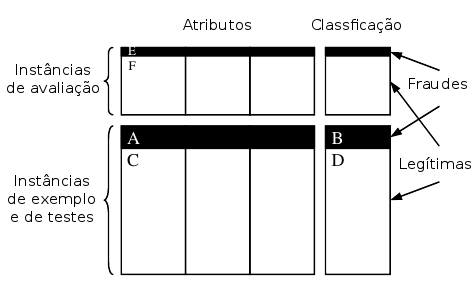
\includegraphics[width=0.75\textwidth]{img/fraud-data.png}
    \vspace{0.5cm}
    \\ Fonte: \cite{Phua2010}.
    \vspace{0.5cm}
\end{figure}

A maioria dos estudos relacionados à detecção de fraude considera a detecção de \emph{outliers} como uma ferramenta principal de detecção \cite{Aral2011}. Existem muitos métodos aplicados à detecção de fraude: auditoria, sistemas especialistas, lógica nebulosa (\emph{fuzzy}), redes neurais, reconhecimento de padrões, árvores de decisão, regressão, etc \cite{Huang2010}. Considerando os dados divididos conforme a figura \ref{fig:fraud_data}, as duas técnicas mais usadas são:

\begin{enumerate}[a)]
\item Dados para treinamento classificados (A + B + C + D) processados por um algoritmo supervisionado.
\item Instâncias legais (C) processadas por um algoritmo semi-supervisionado.
\end{enumerate}

Algoritmos supervisionados examinam as instâncias previamente classificadas (A + B + C + D) para identificar matematicamente os padrões presentes nas classificadas como fraudulentas. Os algoritmos mais utilizados nessa categoria são as redes neurais. Outros algoritmos incluem máquinas de vetores de suporte (\emph{support vector machine}, SVM), árvores de decisão e raciocínio baseado em casos. Para aumentar a eficácia dos métodos supervisionados, esses algoritmos podem ser aplicados em sequência. Também podem ser combinados resultados de bancos de dados distintos.

Algoritmos não-supervisionados atuam sobre dados não classificados (A + C + E + F), e o seu objetivo é agrupar os dados em padrões, para que estes sejam mais facilmente analisados, combinando a detecção humana e a computação da máquina. Exemplos desses algoritmos são redes neurais não supervisionadas, análise de ligações (\emph{link analysis}) e mineração de grafos (\emph{graph mining}).

A combinação de dois ou mais algoritmos supervisionados, ou de algoritmos supervisionados e não-supervisionados, chamados de algoritmos híbridos, é uma grande área de pesquisa. Também são utilizados algoritmos supervisionados em bancos de dados que contêm apenas instâncias legais (C). Regras são geradas e testadas na base de dados, e aquelas que identificam padrões nesses dados são descartadas. Esses algoritmos são chamados de semi-supervisionados, porque apesar de não fazerem distinção entre dados legais e ilegais, os dados ainda necessitam ser classificados para que sejam utilizados no seu treinamento.

Autores como \citeauthor{Phua2010} fazem muitas críticas ao uso de dados previamente classificados para o treinamento dos sistemas \cite{Phua2010}. A classificação atrasa o processo de detecção, aumenta o tempo de reação a novos tipos de fraudes e pode ser cara e difícil de se obter. Pode ainda ser incorreta, tendenciosa e expor dados sigilosos, dependendo do tipo de aplicação. Assim, instâncias de treinamento e avaliação (A + C + E + F, sem classificações) devem ser combinadas e processadas por um algoritmo não-supervisionado, detectando regras, pontuações ou anomalias visuais nos dados avaliados.

Um sistema que detecte e reporte uma fraude muito tempo depois de ela ter ocorrido permite que o fraudador consiga causar um dano substancial. Em geral, esse tempo de resposta de um sistema a partir do momento em que uma fraude é concretizada até a sua detecção é crucial para a eficácia do sistema em de fato proteger o ambiente em que é inserido.

Os sistemas de detecção podem ser divididos em dois tipos gerais, denominados \emph{on-line} e \emph{off-line}, enquanto alguns incorporam características dos dois modelos e outros têm um processo distinto para ambos, que interagem entre si para gerar o resultado final.

\section{Considerações finais}

A detecção de fraude é uma área que pode ser muito aprimorada através da utilização de sistemas computacionais. No entanto, a implementação de um sistema para detecção de fraude é complexa, devido às peculiaridades dessa área: os dados utilizados são sensíveis e esparsos, ocorrências de fraude são raras, comparadas ao grande volume de dados de transações legítimas nas bases de dados. Outro fator importante é que o sistema deve ser adaptável, já que os fraudadores aprimoram constantemente os seus métodos.

Além disso, a detecção, como parte do processo de controle de fraude, deve estar integrada aos outros processos, como a obtenção e segurança dos dados e a divulgação dos resultados. Todos esses processos devem estar em constante funcionamento para que a detecção e a contenção da fraude sejam efetivas, evitando o máximo de danos possível. O sistema de detecção deve fornecer informações suficientes para que a instância possa ser analisada por um especialista para atestar se trata-se realmente de uma fraude. Também é importante que possa haver uma forma de otimização para que o sistema possa ser adaptado aos requisitos da detecção de fraude. Em especial, o número de falsos negativos deve ser o mínimo possível.

Busca-se constantemente aprimorar e adaptar as técnicas tradicionais da mineração de dados para a detecção de fraude. Uma área que oferece uma interessante inspiração é a biologia. Em especial, a imunologia trabalha com cenários muito semelhantes aos sistemas de detecção. Nos próximos dois capítulos, serão apresentados os algoritmos inspirados no sistema imunológico natural e os benefícios que eles podem trazer para os sistemas de detecção.
